%%%%%%%%%%%%%%%%%%%%%%%%%%%%%%%%%%%%%%%%%
% Wenneker Assignment
% LaTeX Template
% Version 2.0 (12/1/2019)
%
% This template originates from:
% http://www.LaTeXTemplates.com
%
% Authors:
% Vel (vel@LaTeXTemplates.com)
% Frits Wenneker
%
% License:
% CC BY-NC-SA 3.0 (http://creativecommons.org/licenses/by-nc-sa/3.0/)
% 
%%%%%%%%%%%%%%%%%%%%%%%%%%%%%%%%%%%%%%%%%

%----------------------------------------------------------------------------------------
%	PACKAGES AND OTHER DOCUMENT CONFIGURATIONS
%----------------------------------------------------------------------------------------

\documentclass[11pt]{scrartcl} % Font size

%%%%%%%%%%%%%%%%%%%%%%%%%%%%%%%%%%%%%%%%%
% Wenneker Assignment
% Structure Specification File
% Version 2.0 (12/1/2019)
%
% This template originates from:
% http://www.LaTeXTemplates.com
%
% Authors:
% Vel (vel@LaTeXTemplates.com)
% Frits Wenneker
%
% License:
% CC BY-NC-SA 3.0 (http://creativecommons.org/licenses/by-nc-sa/3.0/)
% 
%%%%%%%%%%%%%%%%%%%%%%%%%%%%%%%%%%%%%%%%%

%----------------------------------------------------------------------------------------
%	PACKAGES AND OTHER DOCUMENT CONFIGURATIONS
%----------------------------------------------------------------------------------------

\usepackage{amsmath, amsfonts, amsthm} % Math packages

\usepackage{listings} % Code listings, with syntax highlighting
\usepackage[english]{babel} % English language hyphenation
\usepackage{float}
\usepackage{graphicx} % Required for inserting images
\usepackage{caption}
\graphicspath{{Figures/}{./}} % Specifies where to look for included images (trailing slash required)

\usepackage{booktabs} % Required for better horizontal rules in tables

\numberwithin{equation}{section} % Number equations within sections (i.e. 1.1, 1.2, 2.1, 2.2 instead of 1, 2, 3, 4)
\numberwithin{figure}{section} % Number figures within sections (i.e. 1.1, 1.2, 2.1, 2.2 instead of 1, 2, 3, 4)
\numberwithin{table}{section} % Number tables within sections (i.e. 1.1, 1.2, 2.1, 2.2 instead of 1, 2, 3, 4)

\setlength\parindent{0pt} % Removes all indentation from paragraphs

\usepackage{enumitem} % Required for list customisation
\setlist{noitemsep} % No spacing between list items

%----------------------------------------------------------------------------------------
%	DOCUMENT MARGINS
%----------------------------------------------------------------------------------------

\usepackage{geometry} % Required for adjusting page dimensions and margins

\geometry{
	paper=a4paper, % Paper size, change to letterpaper for US letter size
	top=2.5cm, % Top margin
	bottom=3cm, % Bottom margin
	left=3cm, % Left margin
	right=3cm, % Right margin
	headheight=0.75cm, % Header height
	footskip=1.5cm, % Space from the bottom margin to the baseline of the footer
	headsep=0.75cm, % Space from the top margin to the baseline of the header
	%showframe, % Uncomment to show how the type block is set on the page
}

%----------------------------------------------------------------------------------------
%	FONTS
%----------------------------------------------------------------------------------------

\usepackage[utf8]{inputenc} % Required for inputting international characters
\usepackage[T1]{fontenc} % Use 8-bit encoding
\usepackage{adforn}

\usepackage{fourier} % Use the Adobe Utopia font for the document

%----------------------------------------------------------------------------------------
%	SECTION TITLES
%----------------------------------------------------------------------------------------

\usepackage{sectsty} % Allows customising section commands

\sectionfont{\vspace{6pt}\centering\normalfont\scshape} % \section{} styling
\subsectionfont{\normalfont\bfseries} % \subsection{} styling
\subsubsectionfont{\normalfont\itshape} % \subsubsection{} styling
\paragraphfont{\normalfont\scshape} % \paragraph{} styling

%----------------------------------------------------------------------------------------
%	HEADERS AND FOOTERS
%----------------------------------------------------------------------------------------

\usepackage{scrlayer-scrpage} % Required for customising headers and footers

\ohead*{} % Right header
\ihead*{} % Left header
\chead*{} % Centre header

\ofoot*{} % Right footer
\ifoot*{} % Left footer
\cfoot*{\pagemark} % Centre footer
 % Include the file specifying the document structure and custom commands

%----------------------------------------------------------------------------------------
%	TITLE SECTION
%----------------------------------------------------------------------------------------

\title{	
	\normalfont\normalsize
	\textsc{Ca' Foscari University of Venice}\\ % Your university, school and/or department name(s)
	\vspace{25pt} % Whitespace
	\rule{\linewidth}{0.5pt}\\ % Thin top horizontal rule
	\vspace{20pt} % Whitespace
	{\huge A Blockchain Application - Report}\\ % The assignment title
	\vspace{12pt} % Whitespace
	\rule{\linewidth}{2pt}\\ % Thick bottom horizontal rule
	\vspace{12pt} % Whitespace
}

\author{\hspace{-0.8cm} \parbox{4cm}{\centering
  Sandro Baccega\\ 865024} \parbox{4cm}{\centering
  Diletta Olliaro\\ 855957} \parbox{4cm}{\centering
  Giacomo Zanatta\\ 859156} \parbox{4cm}{\centering Giulio Zausa\\ 870040} } % Your name



\date{\vspace{20pt}\today} % Today's date (\today) or a custom date

\begin{document}

\maketitle % Print the title



\section{Introduction}

In this report we are going to present the created blockchain application and to study its performance through the analysis of the results of different benchmarks carried on with the Tsung stress testing tool.

\subsection{Hardware}
The server runs inside a native Linux Docker Container. The underlying host is a Linux machine with the following hardware:
\begin{itemize}
\item[\adforn{43}] CPU: Intel Core i5-2520M 2.5 GHz, 2 cores and 4 threads, 3072 KB L1 Cache
\item[\adforn{43}] RAM: 5828.1MB DDR3
% \item[\adforn{43}] Disk: SanDisk 256 GB SATA SSD
\item[\adforn{43}] Disk: SATA Seagate ST160LT000 160GB 7200 RPM 16MB Cache
\item[\adforn{43}] Network: Intel 82579LM 1 Gbps Wired Ethernet
\end{itemize}

\subsection{Software}

The host is running Ubuntu 20.04 as Operating System, while the application is deployed using Docker. 
This allows us to easily manage deployments and eventual horizontal scaling by spawning multiple nodes. 
Even if our application runs in a Docker container, this will not compromise the performance since it will run on a native Linux host. 
We choosed Docker to future-proof our application, since it will make the deploy of a node in the application's network easy, because it will not require to install any dependencies in the hosting system and it will not have any problem with the versions of those dependencies, saving us a lot of time in the long run.

\section{First Task}

Develop a web application based on the blockchain technology, meaning that in practice we are going to create a non-modifiable database of flying statistics. In the blockchain we must be able to: 
% LOL
\begin{itemize}
\item[\adforn{43}] Add a new transaction
\item[\adforn{43}] Retrieve a transaction based on the transaction ID
\item[\adforn{43}] Retrieve all the transactions of a block
\end{itemize}

Moreover the mining operation should be invoked automatically every minute. 

The web application should also allow the following operations:
\begin{itemize}
\item[\adforn{43}] Add a new record to the chain
\item[\adforn{43}] Query the status of a flight given the flight number and the date
\item[\adforn{43}] Query the average delay of a flight carrier in a certain interval of time
\item[\adforn{43}] Given a pair of cities A and B, and a time interval, count the number of flights connecting city A to city B
\end{itemize}

\subsection{Implementation}

\begin{figure}[h]
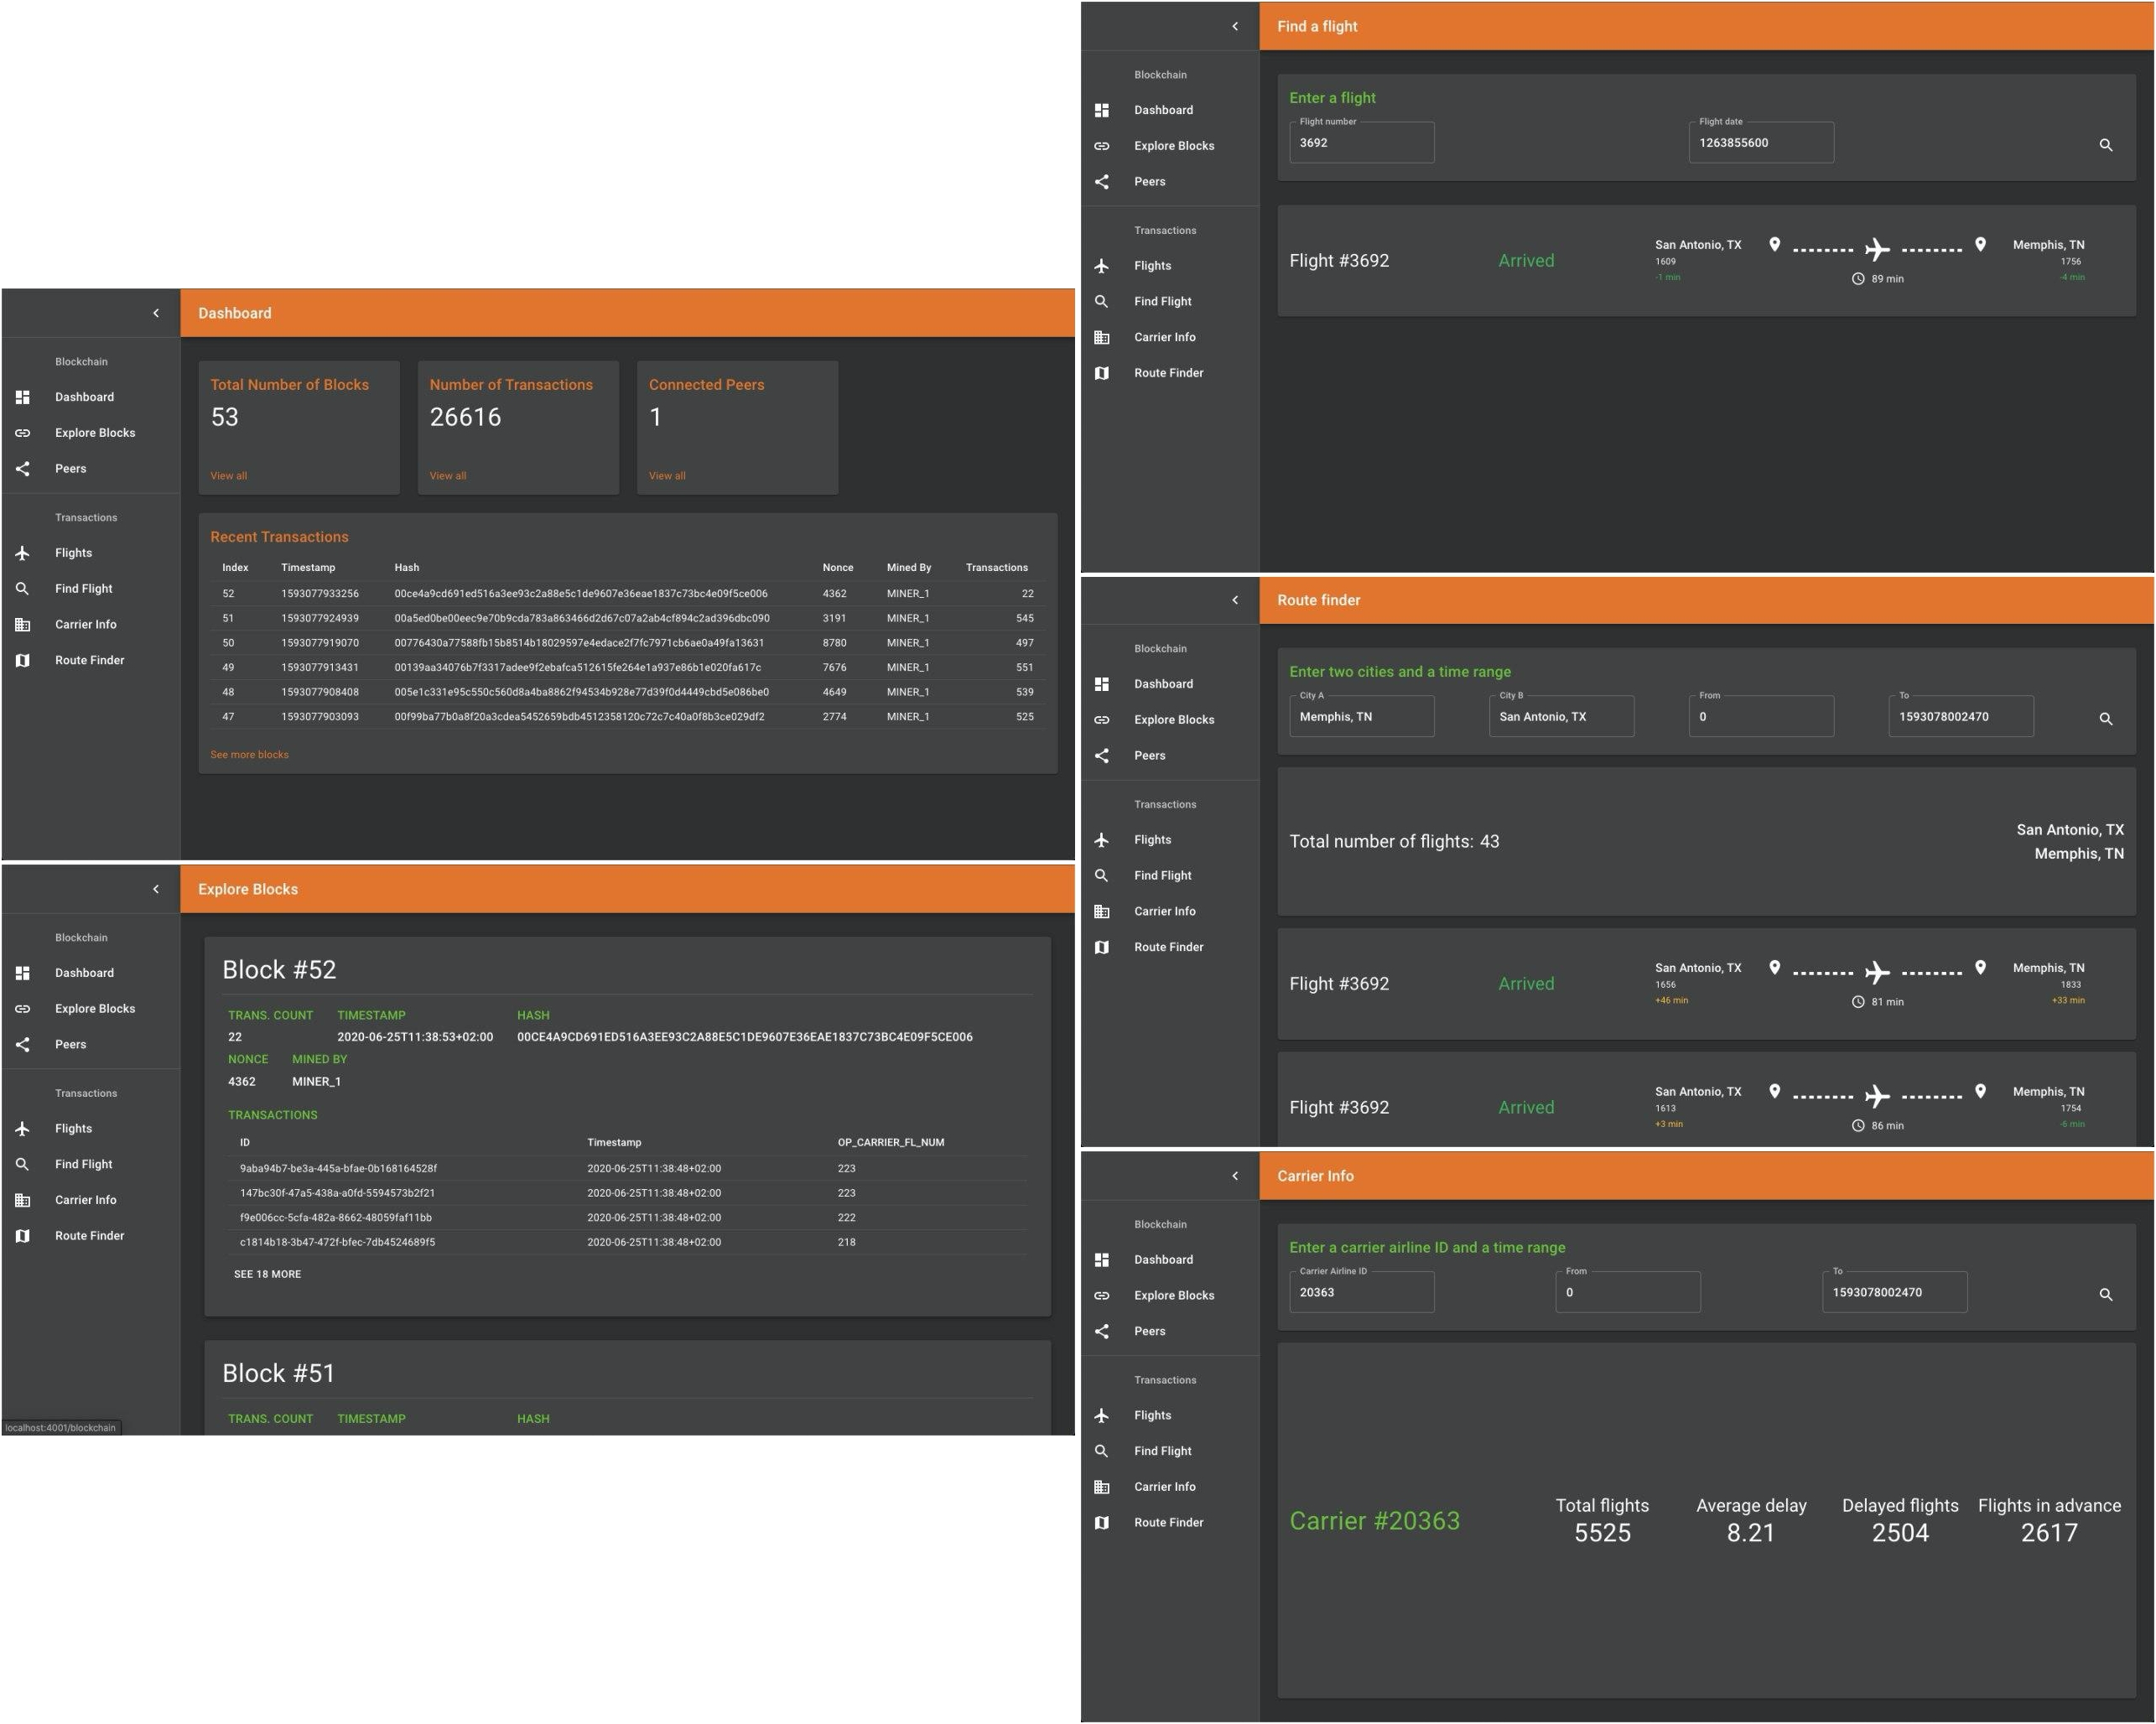
\includegraphics[width=9cm]{Images/frontend.png}
\centering
\caption{The Blockchain React App UI}
\label{fig:frontend}
\end{figure}

For implementing the \textit{blockchain} system we used \textbf{NodeJS} with TypeScript. NodeJS is a server runtime that runs JavaScript code. The main feature of NodeJS is its \textbf{Event Queue} \textit{(libuv)}: every IO operation is enqueued in a FCFS queue and processed by multiple threads (figure \ref{fig:eventloop}). The application logic, though, remains single-threaded. In this way the requests are processed with a FCFS policy, as we have seen also from the benchmark data.

\begin{figure}[h]
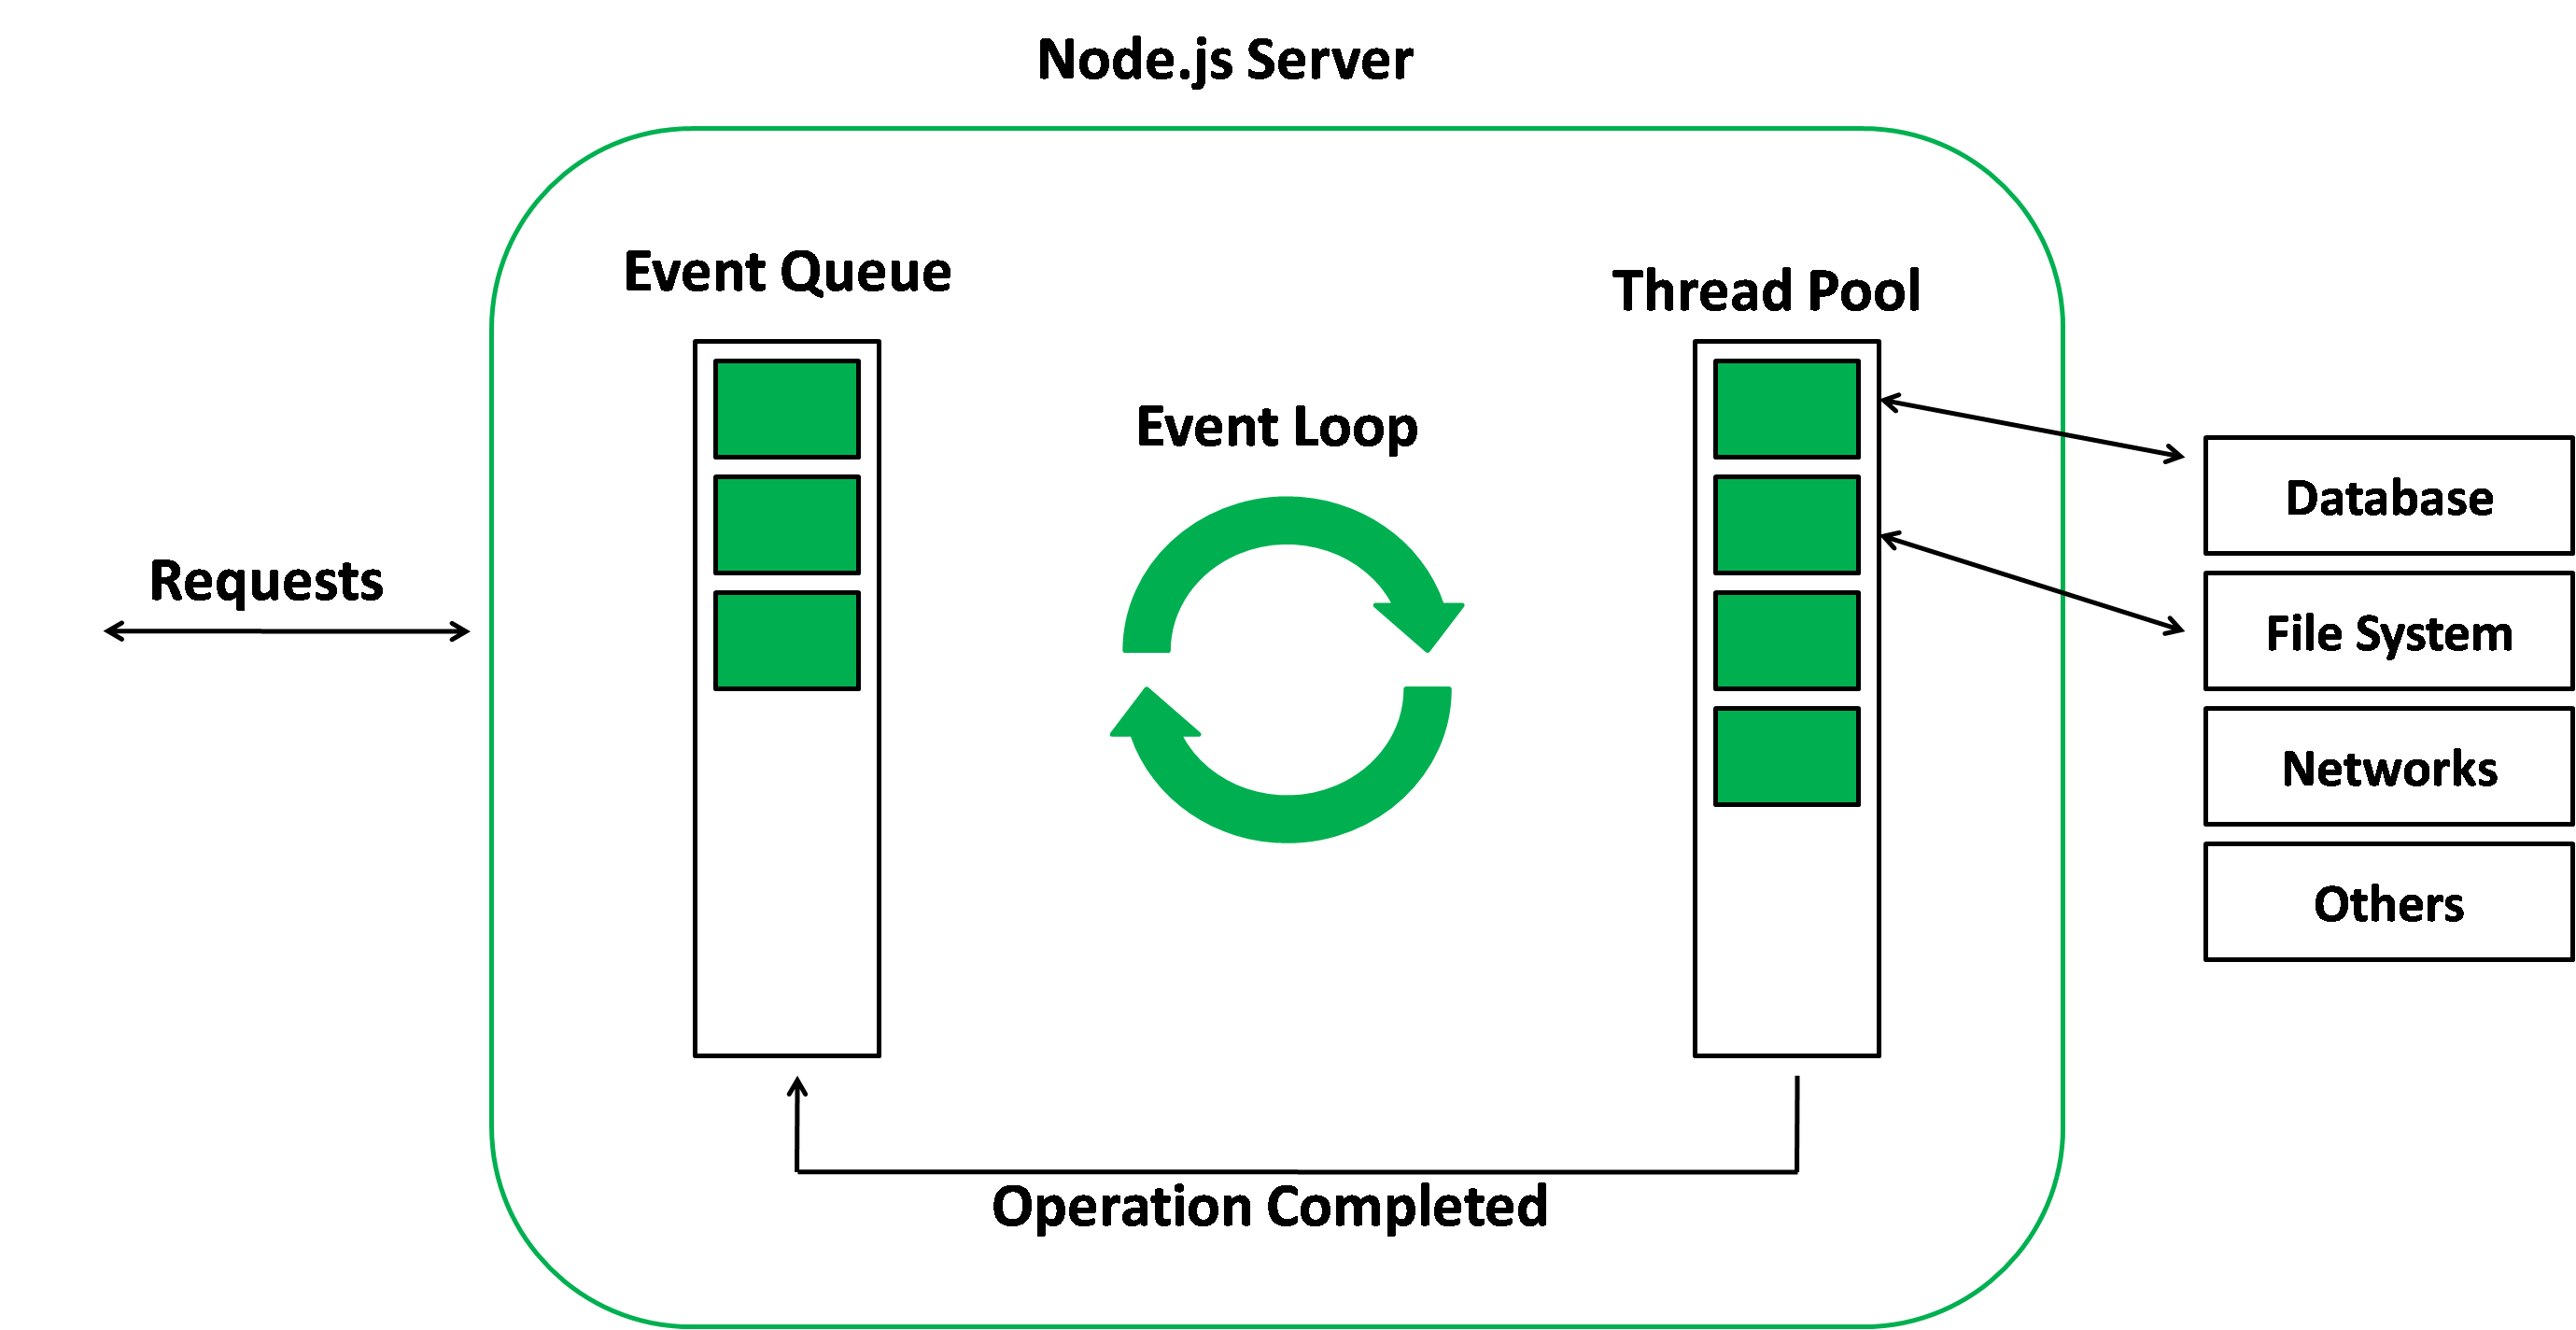
\includegraphics[width=8cm]{Images/eventloop.png}
\centering
\caption{The Node.JS Event Loop}
\label{fig:eventloop}
\end{figure}


The blockchain is actually stored in a LevelDB database. LevelDB is a simple embedded key-value storage engine that provides an ordered mapping from string keys to string values. Moreover, it provides basic operations like:
\begin{itemize}
\item[\adforn{43}] \texttt{put(key,value)} that insert value with the given key inside the DB (if the value is already defined, it will override its value with the new one)
\item[\adforn{43}] \texttt{get(key)} that given a key, it will return the associated value (or null if the value is not in the DB)
\item[\adforn{43}] \texttt{delete(key)} that removes the given key (if present) from the DB.
\end{itemize}

The blockchain data is replicated in every node of the system. When a new node starts, it will reach out to a known node to be registered in the network. Every node keeps the list of peers and they exchange their list with each others to keep track of new or lost peers.

Once a node has entered the network it starts a procedure called \textit{Initial Block Download}: it asks for the longest chain and it downloads the missing blocks from a random peer.

Once it has downloaded the whole blockchain, the node is said to be active and it can perform queries or add new transactions. Every node tries to mine a new block in an asynchronous way. When a node mines a block it announces it to all the others nodes in the system.

Each node consists of two services: front-end and back-end. The front-end is a static React web app (figure \ref{fig:frontend}) that handles the user input and communicate with an API to the back-end in order to fetch the data it needs. In our particular case, when a user wants to add a flight into the system, it can access the front-end interface, which provides a form, and insert the data. Once the form is correctly filled, the flight is inserted in a queue and it waits until a node in the network mines a block containing all the transactions that are currently in the queue. Using the front-end application a user can also make queries to fetch routes and flights. 

\section{Second Task}

After we implemented our application we wanted to analyse its performance and scalability properties. In order to do so, we used \textit{Tsung}\footnote{Tsung is an high-performance benchmark framework.} to perform some benchmarks.

To perform the benchmarks we used two different machines: the server (described previously) and another identical Linux machine, directly connected via wired network and a Gigabit Ethernet switch. We have done this to avoid performance drops due to the benchmark software.


\paragraph*{1. Imagine the system as a monolithic queue and measure its expected service time and its second moment.} \mbox{}\\\\ 

To find the queue's expected service time and its second moment we performed a benchmark test using Tsung with a single customer in the system. The customer is supposed to make a query, wait for the answer and then leave the system, performing a closed test. This kind of setup ensures that every request is independent from the previous ones. 
The first step was to run a single test with this setup, requesting every endpoint of the server, to decide which query was the slowest. In this way we could use just that one for our benchmarks since it would represent a good indicator for a heavy load.
We did this because if we used the fastest query for the benchmark we would produce a underestimated result. 
The queries had the following response times:

\begin{table}[H]
\centering
\begin{tabular}{c|c}
\multicolumn{1}{l|}{Request} & \multicolumn{1}{l}{Mean Service Time} \\ \hline
tr\_blockLast & 4.94 msec \\
tr\_blocks20 & 0.45 sec \\
tr\_carriers & 2.45 sec \\
tr\_chainInfo & 3.96 msec \\
tr\_flights & 2.45 sec \\
tr\_peers & 1.60 msec \\
tr\_route & 2.48 sec \\
\end{tabular}
\end{table}

We can see that the heaviest query is the one that states: \textit{"given a pair of cities A and B, and a time interval, count the number of flights connecting city A to city B"}.\\

The second step we did was to run 30 separate tests like the one before, choosing randomly the parameters for the query (to avoid biased results like before). In this way we were able to obtain the expected service time and its variance, which resulted to be, respectively 2330.0 ms and 5389.028 ms.
Notice that we were able to retrieve the expected service time from the response time, since having just one customer at the time in a system is in practice the same as setting to zero the waiting time, consequently the response time must correspond only to the service time.

\paragraph*{2. Perform the test as open system with different workload intensities: 0.3L, 0.5L, 0.8L, 0.85L, where L is the maximum arrival rate determined from the expected service time estimated at point 1. Compare the measures with the lines predicted by the M/G/1 and M/G/1/PS queueing systems and discuss the results.} \mbox{}\\\\

The maximum arrival rate is given by the maximum throughput of the bottleneck (in this particular case we are considering to have just 1 station, so we know which one is the bottleneck) and the maximum throughput at the bottleneck is given by its service rate.

We want to compute the theoretical values of expected response time and expected number of jobs supposing we have an M/G/1 or an M/G/1/PS queue, so that then we can compare these measures with the ones obtained from the benchmarks.

We know in general that the response time is given by the expected waiting time plus the service time, in particular:

\begin{itemize}
\item[\adforn{43}] In the M/G/1 setting the expected waiting time is given by $$E[W]=\dfrac{\rho+\lambda\mu\sigma^2}{2(\mu-\lambda)}$$ and assuming stability the expected service time is given by $\dfrac{1}{\mu}$, therefore:
$$\overline{R}=E[W]+\dfrac{1}{\mu} .$$

This means that in this setting the expected number of jobs is given by the expected number of jobs in the waiting room plus the ratio of users being served, i.e.

\begin{align*}
E[N_W] &= \lambda E[W]\\
E[N] &= E[N_W]+\dfrac{\lambda}{\mu}
\end{align*}

\item[\adforn{43}] In the M/G/1/PS setting we know expected response time and number of jobs do not depend on the variance and correspond to the measures we use for M/M/1 systems; i.e.:

\begin{align*}
\overline{R} &= \dfrac{1}{\mu-\lambda}\\
\overline{N} &= \dfrac{\rho}{1-\rho}
\end{align*}

\end{itemize}

Using this we found the following theoretical data (RespTime and NumJobs stand for the expected response time and the expected number of jobs, respectively):

\begin{table}[H]
\centering
\begin{tabular}{c|c|c|cc}
\multicolumn{1}{l|}{}         & \multicolumn{2}{c|}{M/G/1}                                                        & \multicolumn{2}{c}{M/G/1/PS}                                                     \\ \hline
\multicolumn{1}{l|}{Workload} & \multicolumn{1}{l|}{RespTime (ms)} & \multicolumn{1}{l|}{NumJobs} & \multicolumn{1}{l|}{RespTime (ms)} & \multicolumn{1}{l}{NumJobs} \\ \hline
0.3                           & 2829.78                            & 0.36                                         & \multicolumn{1}{c|}{3328.57}       & 0.43                                        \\
0.5                           & 3496.16                            & 0.75                                         & \multicolumn{1}{c|}{4660.0}        & 1.0                                         \\
0.8                           & 6994.63                            & 2.40                                         & \multicolumn{1}{c|}{11650.0}       & 4.0                                         \\
0.85                          & 8938.22                            & 3.26                                         & \multicolumn{1}{c|}{15533.33}      & 5.67                                       
\end{tabular}
\end{table}

Below, we show the table containing the data found doing benchmarks of our application using Tsung, configuring a load using as arrival rate the workload multiplied by the service time:

\begin{table}[H]
\centering
\begin{tabular}{c|c|c}
\multicolumn{1}{l|}{Workload} & \multicolumn{1}{l|}{RespTime (ms)} & \multicolumn{1}{l}{NumJobs} \\ \hline
0.3                           & 3036.72                            & 0.39                         \\
0.5                           & 3716.63                            & 0.83                         \\
0.8                           & 6981.09                            & 2.13                         \\
0.85                          & 9562.70                            & 3.62                        
\end{tabular}
\end{table}

\begin{figure}[H]
\centering
\includegraphics[width=15cm]{Images/respTimes.png}
\caption{Mean response time}
\end{figure}

\begin{figure}[H]
\centering
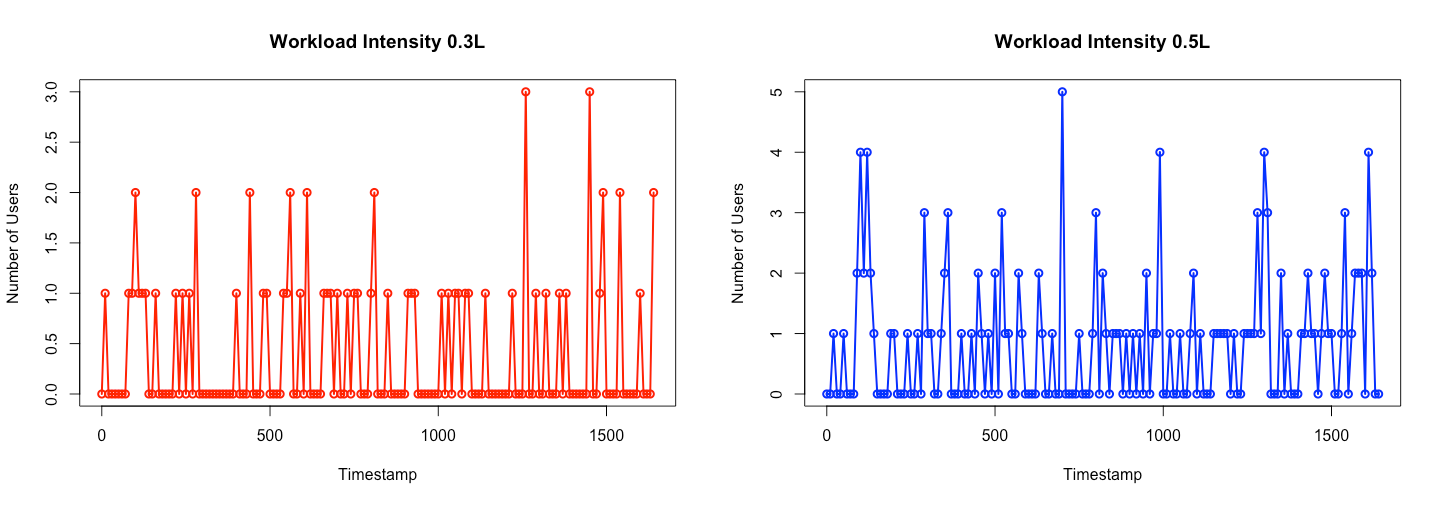
\includegraphics[width=15cm]{Images/user35side.png}
\end{figure}

\begin{figure}[H]
\centering
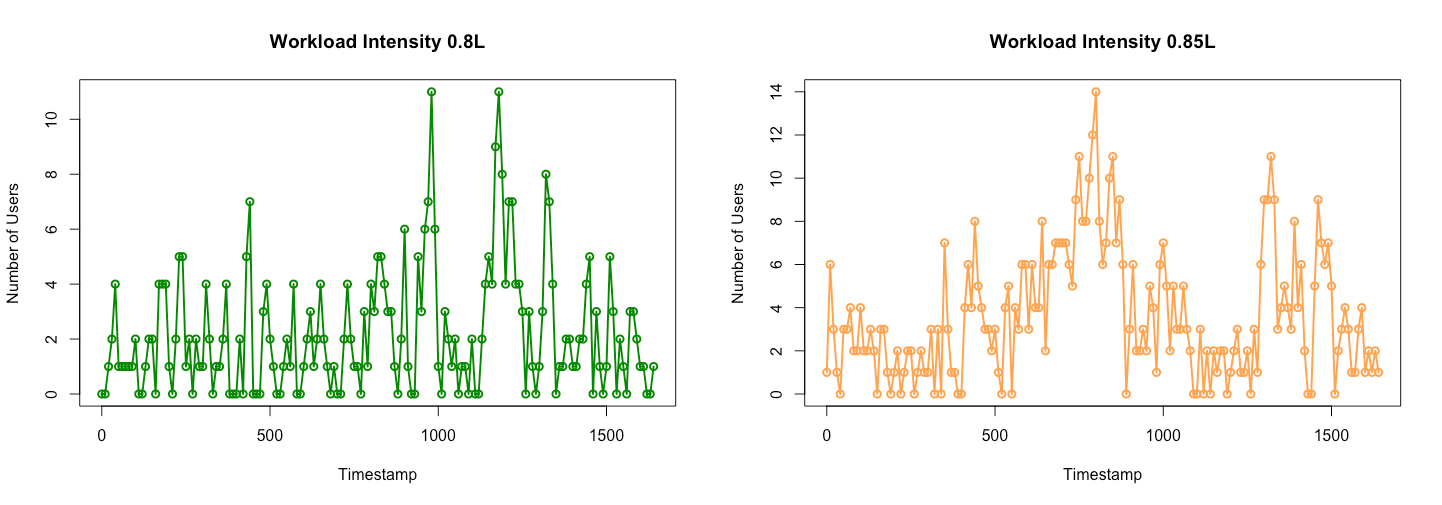
\includegraphics[width=15cm]{Images/user858side.png}
\end{figure}


Comparing the two tables we can notice that our empirical measurements are closer to the M/G/1 theoretical values than the M/G/1/PS ones. This can be also explained technically by the architecture of the server: since we are using Node.JS, every incoming request is added to the JavaScript event queue by \textit{libuv}, waiting to be processed by our event handlers. Since the event queue is processed with a FCFS policy, our requests queue is following that policy too.


\paragraph*{3. Propose a queueing network model of your application where you distinguish at least three stations: disk, processor and a station modeling the thinking time of the requests. Parametrize the queueing network based on the measurements you can do on your application.} \mbox{}\\\\

We modelled our queuing network based on considerations from our implementation:

\begin{itemize}
\item[\adforn{43}] Once a request is received, a disk read is immediately enqueued to fetch the blocks from the database;
\item[\adforn{43}] All the blocks are fetched from the LevelDB database, reading from the disk;
\item[\adforn{43}] Once all blocks are read, they are filtered and processed using a blocking CPU process.
\end{itemize}

Therefore, the system can be modelled as a three-stations closed-loop queuing network (figure \ref{fig:img1}).

\begin{figure}[H]
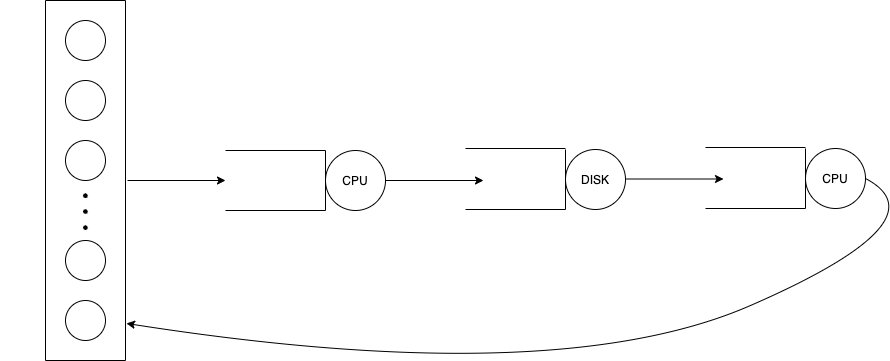
\includegraphics[width=10cm]{Images/img1.png}
\centering
\caption{Model with three stations}
\label{fig:img1}
\end{figure}

This approach, however, it's problematic due to the nature of Node.JS, since it becomes difficult to benchmark the utilization of the two CPUs stations. For this reason we choose a simpler model (figure \ref{fig:img2}), with only the second CPU station, since the time required to read the request and start the disk read (the first station's task) is much lower than the time required to wait for the read and perform the filtering and aggregation (the second station's task).

\begin{figure}[h]
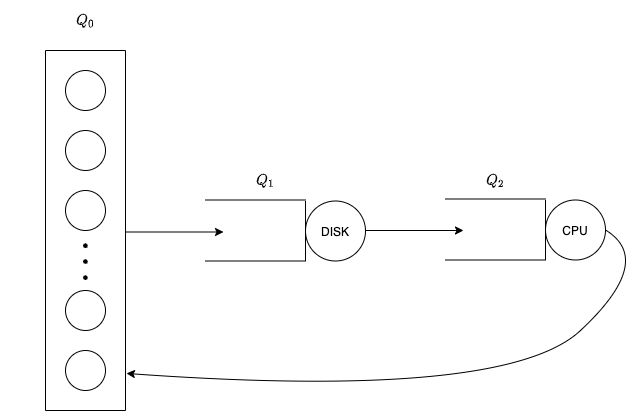
\includegraphics[width=10cm]{Images/img2.png}
\centering
\caption{Model with two stations}
\label{fig:img2}
\end{figure}

As \textbf{thinking time} we have choosen a resonable value of $10$ seconds: once an user receieves the results from the server, we expect him to spend this time to read them before making another request.\\

To perform further analysis on this model, we needed to find the service times of the two stations. To do so we performed another closed-loop benchmark with Tsung, using a single user and no thinking time. While performing the benchmark we used Node.JS Performance Timings to monitor how much time was spent in every part of the code. To check the disk response time we measured for each request the time spent in Unix file access primitive calls. After performing 200 requests with Tsung ($\approx 10$ minutes) we aggregated our results and we computed the average time spent for disk requests and for CPU usage, in percentage:

% While performing the benchmark we used the \textbf{iostat} tool to monitor the usage of the disk and the CPU. Using the command \texttt{iostat -x 30} we sampled the utilization of the system every 30 seconds. To find the utilization of the disk we used the \texttt{\%iowait} field, since it represents the percentage of time waiting for an IO device. To find the utilization of the CPU we used the \texttt{\%user} field. After reading 50 samples (25 minutes) we calculated an average of the two utilizations, performing a normalization to $100\%$:

\begin{table}[H]
\centering
\begin{tabular}{c|c}
\multicolumn{1}{l|}{\%Disk} & \multicolumn{1}{l}{\%CPU} \\ \hline
$98.21\%$ & $1.79\%$\\
\end{tabular}
\end{table}

Since we know from the previous benchmarks the average value of the total service time (2445ms) we can multiply this with the previously found utilizations, finding the average service time for the disk and for the CPU data aggregation:

\begin{table}[H]
\centering
\begin{tabular}{c|c|c}
\multicolumn{1}{l|}{Thinking Time ($Q_0$)} & \multicolumn{1}{l|}{Disk Time ($Q_1$)} & \multicolumn{1}{l}{CPU Time ($Q_2$)} \\ \hline
$10,000$ ms	&  $2401.19$ ms	& $43.75$ ms \\
\end{tabular}
\end{table}


\paragraph*{4. Determine the bottleneck of the system and use the operational analysis to determine the maximum level of multiprogramming. (Choose a reasonable expected thinking time)} \mbox{}\\\\

A good practice at this point is to find what can be improved in the system to make performances better. To do so it is necessary to find where critical issues start i.e. to find the bottleneck of the system. To discover which station represent the bottleneck of the system we need to consider both the speed and the relative  visit ration at each station i.e. we need to compute the service demands at each station. In the previous paragraph we were able to retrieve the service times which lead us  to the following service rates:

\begin{align*}
\mu_{DISK} &= \dfrac{1}{2401.19}\ ms=0.00042\ ms\\
\mu_{CPU} &= \dfrac{1}{43.75}\ ms=0.0229\ ms
\end{align*}

At this point to find the relative visit ratios, considering that we are in a closed system, we had to model the system of traffic equations that we show below:

$$\begin{cases} e_0=e_2\\ e_1=e_0\\ e_2=e_1\end{cases}$$

Since the system is under-determined we need to fix a reference station and compute the  results with respect to it. We choose the reference station to  be $Q_0$ i.e. the  delay station, consequently we set $e_0 = 1$. Accordingly the solution of the system is given by:

$$\begin{cases} e_0=1\\ e_1=1\\ e_2=1\end{cases}$$

Now, we do the following  computations to retrieve the service demands:

$$D_{DISK}=\dfrac{1}{0.00042}=2402.19\qquad D_{CPU}=\dfrac{1}{0.0229}=43.75$$

The station with the highest service demand is the bottleneck, so we can recognize that is the \textbf{disk}. This makes sense because of how the query is implemented: every time a query is performed the whole blockchain is read, and this is an expensive operation.

Now, we are interested in discovering what could be our maximum level of multiprogramming, to do so we can use some theoretical result deriving from an operational analysis on the upper bounds of the throughput.


We know these bounds are given by $$X\leq \mathrm{min}\bigg(\dfrac{1}{D_b}, \dfrac{N}{D+Z}\bigg)$$

where $D$ is the sum of all the service demands and $D_b$ is the service demand at the bottleneck. This holds because:

\begin{itemize}
\item[\adforn{43}] we know the bottleneck establishes the maximum throughput of the system so the throughput of  the system is going to be lower than or equal to this, i.e. $$X\leq \dfrac{1}{D_B}$$ 
\item[\adforn{43}] moreover supposing we have a system with no waiting time then the response time would be equal to the sum of the service demands plus the thinking time; because of the lack of waiting time the response time above ($\widetilde{R}$) will be lower than the actual expected one ($\overline{R}$), accordingly thanks to Litlle's law we can state the following: $$X=\dfrac{N}{\overline{R}}\leq \dfrac{N}{\widetilde{R}}=\dfrac{N}{D+Z}$$
\end{itemize}

consequently as we stated above $X\leq\bigg(\dfrac{1}{D_b}, \dfrac{N}{D+Z}\bigg)$.\\

According to this reasoning we find: $$\widetilde{N}_{\mathrm{opt}}=\dfrac{D+Z}{D_b}=\dfrac{2445.94+10000}{2402.19}=5.18\approx 5\ \mathrm{interactive\ users}$$

In fact, we tried to perform a benchmark with 7 interactive users and we noticed a big degradation in the performances, especially in the response times that resulted to be even three times bigger.


\paragraph*{5. Use JMT to study the queueing network and evaluate with MVA an action to increase the maximum level of multiprogramming of the system.} \mbox{}\\\\

We already used the technique of finding the two asyntotes crossing point to estimate the maximum level of multiprogramming, but performing a mean value analysis we can do even better. To perform the MVA we used the Java Modeling Tool\footnote{An open source suite for queueing network modelling and workload analysis}. We set up the parameters so that they represent our model well, then we used the values found in the previous paragraphs. The set up resulted to be as follows:

\begin{figure}[H]
\centering
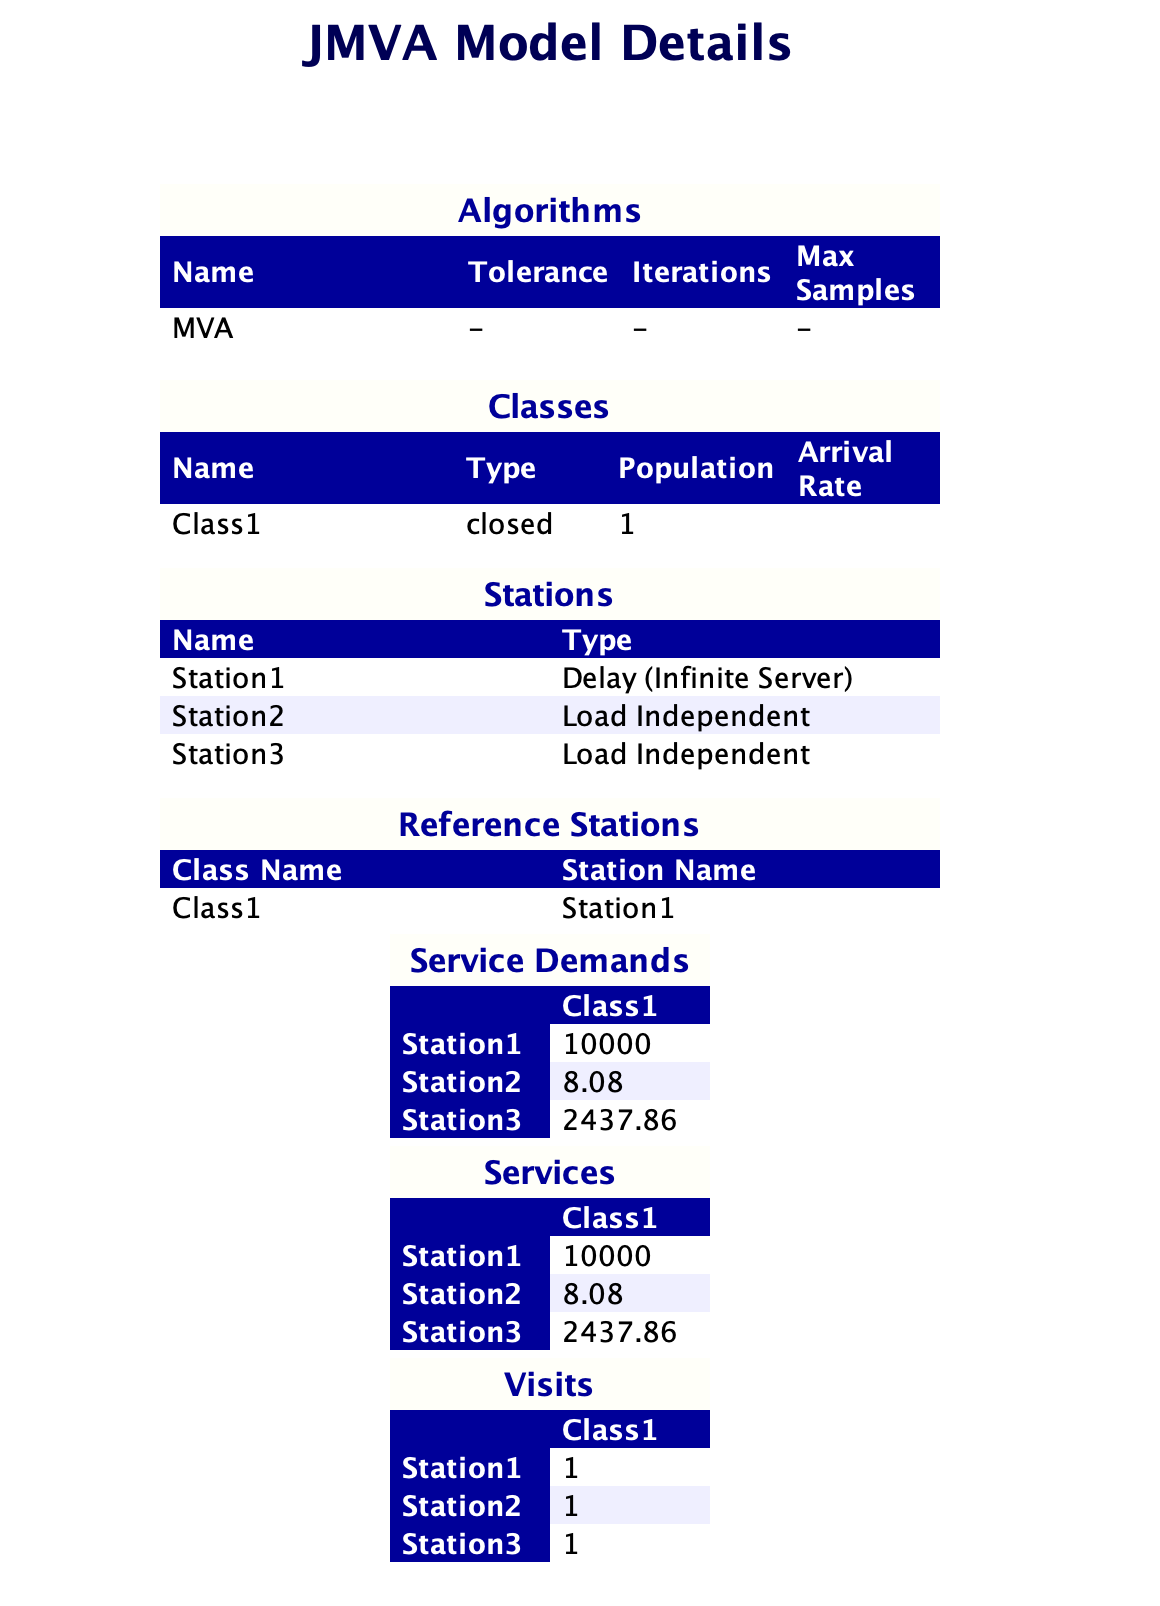
\includegraphics[width=8cm]{Images/JMVAsynopsis.png}
\end{figure}

The results of the analysis were the following graphs. Notice that the red line represents the delay station ($Q_0$), the blue line represents the disk ($Q_1$) and the green line represents the CPU ($Q_3$).\\

From figure \ref{fig:img3} we can see that the throughput of the different stations becomes to be saturated around 8 interactive users, meaning that this will be the actual number of optimal users we can afford to have in our system; without having any deterioration in performances. 

In the graph represented in figure \ref{fig:img5} we have the confirmation that station 2, i.e. the disk, is our bottleneck as a matter of fact when increasing the number of users in the system it is visible they start to accumulate in the station 2 queue.

This can also be noticed looking at figure \ref{fig:img4} where we can see the response time  of the disk increasing quickly and non-linearly while the number of users grows. Whereas the CPU station responds fairly well to the growth of the number of users, and as expected the delay station remains constant.


\begin{figure}[h]
\centering
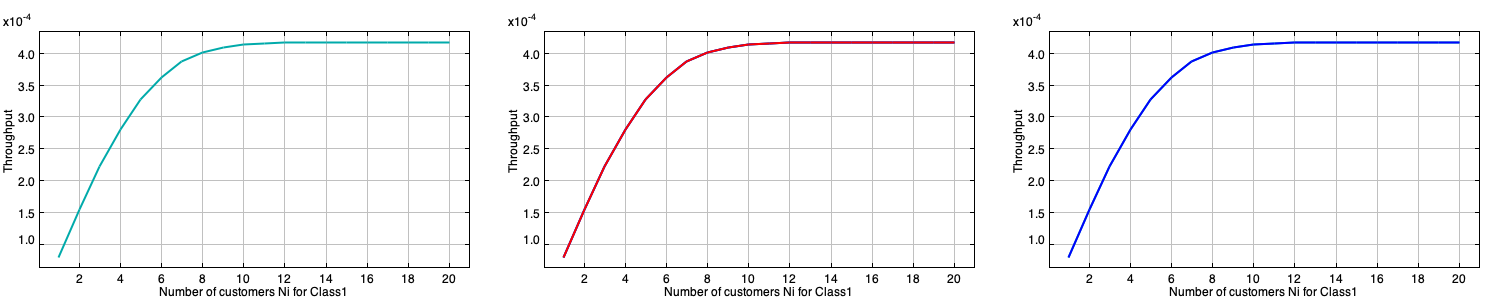
\includegraphics[width=12cm]{Images/JMVAthroughputside.png}
\caption{Throughput for each station}
\label{fig:img3}
\end{figure}

\begin{figure}[h]
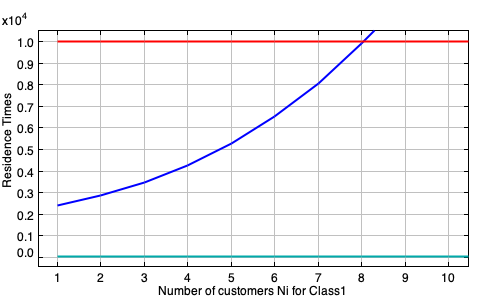
\includegraphics[width=10cm]{Images/JMVAresTimes.png}
\centering
\caption{Response times as the  number  of users increases}
\label{fig:img4}
\end{figure}

\begin{figure}[h]
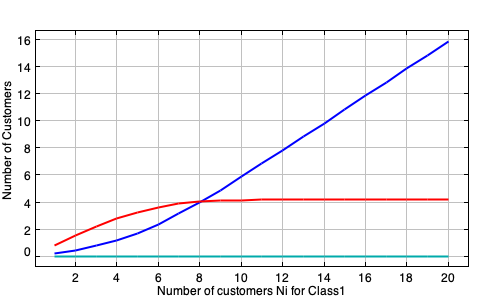
\includegraphics[width=10cm]{Images/JMVAnumUsers.png}
\centering
\caption{Number of customers}
\label{fig:img5}
\end{figure}

This analysis helped us in confirming some of our hypothesis and in being more precise about the maximum number of users we can have in the system. To improve performances and the bottleneck situation we could:

\begin{itemize}
\item[\adforn{43}] Use a Solid State Disk in the server, which would dramatically improve the disk read performance, lowering the disk read service time;
\item[\adforn{43}] Use a better algorithm for database read in the query, employing a cache and/or streaming aggregation on the fly while reading data, without waiting all data to be read;
\item[\adforn{43}] Spawn multiple instances of the server distributing the query workload in different machines.
\end{itemize}

Since our blockchain node application is already designed to be distributed and since the query are read only and we could easily, as we said, use a \textit{Load Balancer} to route every request to a different machine. In this way, assuming zero service time in the load balancer, we could scale linealy the maximum level of multiprogramming of our system, simply increasing the number of active servers. We could deploy this very easily with an container-orchestration system like \textit{Kubernetes} since we are using Docker containers for our application.

\section{Conclusion}

Doing this assignment we learnt many notions about systems modeling and performance analysis that are very important when deploying large system that have to scale well:

\begin{itemize}
\item[\adforn{43}] Always benchmark your application in a proper way when you want to ensure its scalability, planning how many users you expect to have;
\item[\adforn{43}] A solid analytical model is crucial to understand performance patterns and how to read benchmark results properly;
\item[\adforn{43}] Sometimes the bottleneck of your system is not where you expect it to be, and many times it's useful to perform a benchmark \textbf{before} doing any type of premature optimization to the code.
\end{itemize}

We understood that many different considerations and assumptions have to be made even when modeling a simple system. This required us to thoroughly go through the theory we studied and to try many different configurations before actually getting the desired result. Nevertheless, trial and error has been useful to achieve a final model which is reasonable and resembles the theoretical results fairly well.

\end{document}
